\documentclass[fleqn,11pt]{jreport}
\usepackage{mysty}
\usepackage{graphicx}

\begin{document}
\baselineskip 21.5pt

\begin{titlepage}
\vspace*{3cm}
\begin{center}
{\Large\gt 東京都市大学メディア情報学部}\\
\vspace*{0.5cm}
{\Large\bf 2018年度卒業研究}\\
\vspace{1.5cm}

% 論文タイトルが1行の場合
{\huge\bf 自動作曲の研究}\\

% 論文タイトルが2行の場合
%{\huge\bf 自動作曲の}\\
%\vspace{0.5cm}
%{\huge\bf 研究}\\

\vspace{9cm}
{\Large メディア情報学部 情報システム学科 xxxxxxx}\\
{\Large 大野木 俊樹}\\
\vspace*{0.5cm}
{\Large 指導教員 大谷紀子 教授}\\
\end{center}
\end{titlepage}

\pagenumbering{roman}
\tableofcontents
\cleardoublepage

\pagenumbering{arabic}
% 本文のファイルを以下に列挙する
\chapter{はじめに}
あああああああああああああああああああああああああああああああああああああああああああああああああああああああああああああああああああああああああああああああああああああああああああああああああああああああああああああああああああああああああああああああああああああああああああああああ

参考文献はこんな感じで引用します.
\cite{Quinlan96}
\cite{Quinlan89}
\cite{Quinlan93}
\cite{Iba94}
\cite{C50}
\cite{Nakayama00}
\cite{Otani06}
\cite{Otani04}
\cite{Saino88}
\cite{Ishibashi11}
\cite{Ushijima11}


図はこんな風に入れます.

\begin{figure}[tbhp]
\begin{center}
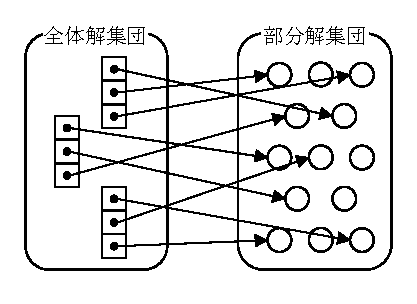
\includegraphics[scale=0.95]{images/se.eps}
\caption{共生進化における2つの集団}
\label{fig:02se}
\end{center}
\end{figure}

図番号は図\ref{fig:02se}のように参照します.

\chapter{○○の現状}
あああああああああああああああああああああああああああああああああああああああああああああああああああああああああああああああああああああああああああああああああああああああああああああああああああああああああああああああああああああああああああああああああああああああああああああああ

\section{あいうえお}
あああああああああああああああああああああああああああああああああああああああああああああああああああああああああああああああああああああああああああああああああああああああああああああああああああああああああああああああああああああああああああああああああああああああああああああああ

\section{かきくけこ}
あああああああああああああああああああああああああああああああああああああああああああああああああああああああああああああああああああああああああああああああああああああああああああああああああああああああああああああああああああああああああああああああああああああああああああああああ


\chapter{ABCシステム}
あああああああああああああああああああああああああああああああああああああああああああああああああああああああああああああああああああああああああああああああああああああああああああああああああああああああああああああああああああああああああああああああああああああああああああああああ

\section{あいうえお}
あああああああああああああああああああああああああああああああああああああああああああああああああああああああああああああああああああああああああああああああああああああああああああああああああああああああああああああああああああああああああああああああああああああああああああああああ

\section{かきくけこ}
あああああああああああああああああああああああああああああああああああああああああああああああああああああああああああああああああああああああああああああああああああああああああああああああああああああああああああああああああああああああああああああああああああああああああああああああ

\chapter{評価実験}
あああああああああああああああああああああああああああああああああああああああああああああああああああああああああああああああああああああああああああああああああああああああああああああああああああああああああああああああああああああああああああああああああああああああああああああああ

\section{あいうえお}
あああああああああああああああああああああああああああああああああああああああああああああああああああああああああああああああああああああああああああああああああああああああああああああああああああああああああああああああああああああああああああああああああああああああああああああああ

\section{かきくけこ}
あああああああああああああああああああああああああああああああああああああああああああああああああああああああああああああああああああああああああああああああああああああああああああああああああああああああああああああああああああああああああああああああああああああああああああああああ

\chapter{考察}
あああああああああああああああああああああああああああああああああああああああああああああああああああああああああああああああああああああああああああああああああああああああああああああああああああああああああああああああああああああああああああああああああああああああああああああああ

\section{あいうえお}
あああああああああああああああああああああああああああああああああああああああああああああああああああああああああああああああああああああああああああああああああああああああああああああああああああああああああああああああああああああああああああああああああああああああああああああああ

\section{かきくけこ}
あああああああああああああああああああああああああああああああああああああああああああああああああああああああああああああああああああああああああああああああああああああああああああああああああああああああああああああああああああああああああああああああああああああああああああああああ

\chapter{おわりに}
あああああああああああああああああああああああああああああああああああああああああああああああああああああああああああああああああああああああああああああああああああああああああああああああああああああああああああああああああああああああああああああああああああああああああああああああ


\chapter*{謝 辞}
\markboth{謝 辞}{謝 辞}
\addcontentsline{toc}{chapter}{謝 辞}
みんなに感謝いたします.
そうです.みんなに感謝するのです.


\markboth{参考文献}{参考文献}
\bibliographystyle{jsai}
%\bibliographystyle{plain}
\bibliography{mybib}

\appendix
% 付録のファイルを以下に列挙する
\chapter{アンケート用紙}
あああああああああああああああああああああああああああああああああああああああああああああああああああああああああああああああああああああああああああああああああああああああああああああああああああああああああああああああああああああああああああああああああああああああああああああああ

\section{あいうえお}
あああああああああああああああああああああああああああああああああああああああああああああああああああああああああああああああああああああああああああああああああああああああああああああああああああああああああああああああああああああああああああああああああああああああああああああああ

\section{かきくけこ}
あああああああああああああああああああああああああああああああああああああああああああああああああああああああああああああああああああああああああああああああああああああああああああああああああああああああああああああああああああああああああああああああああああああああああああああああ

\chapter{被験者の自由記述}
あああああああああああああああああああああああああああああああああああああああああああああああああああああああああああああああああああああああああああああああああああああああああああああああああああああああああああああああああああああああああああああああああああああああああああああああ

\section{あいうえお}
あああああああああああああああああああああああああああああああああああああああああああああああああああああああああああああああああああああああああああああああああああああああああああああああああああああああああああああああああああああああああああああああああああああああああああああああ

\section{かきくけこ}
あああああああああああああああああああああああああああああああああああああああああああああああああああああああああああああああああああああああああああああああああああああああああああああああああああああああああああああああああああああああああああああああああああああああああああああああ


\end{document}
